% !TeX spellcheck = en_US
\section{Simulation Examples}
{
	\color{red}
\begin{itemize}
	\item Zuerst Sprungantwort
	\item Danach Sweep
\end{itemize}
}

For each proposed ladder type, we assume an example consisting of ten sub-circuits. The resistor, capacitor and inductor values  are equal for all sub-circuits, they are listed in Table \ref{table:simulation_parameters}. As we have equal component values, the triangular matrices for each ladder type are filled with ones and scaled as
\begin{equation*}
	\mathbf{T} = \left(a~b\right) ~ \mathbf{\tilde{T}} \quad \text{with} \quad 
	\mathbf{\tilde{T}} :=
	\begin{pmatrix}
		1 & \ldots & 1 \\
		& \ddots & \vdots \\
		& & 1
	\end{pmatrix} 
	\textbf{.}
\end{equation*}
The multipliers of the scaling $a\cdot b$ are listed in Table \ref{table:triangular_matrix_values}. Hence, we yield the differential equations
\begin{equation}
	(\ell~c)~\mathbf{T} ~ \ddot{z}(t) + (r~c)~\mathbf{T}~ \dot{z}(t) + \mathbf{\tilde{F}}~ z(t) = G~u(t)
\end{equation}
for circuit type (a) (capacitor as shunt), 
\begin{equation}
	\left(\frac{\ell}{r}\right)~\mathbf{T}~ \ddot{z}(t) + \mathbf{\tilde{F}}~\dot{z}(t) + \left(\frac{1}{r~c}\right)~\mathbf{T}~ z(t) = G~\dot{u}(t)
\end{equation}
for circuit type (b) (resistor as shunt) and
\begin{equation}
	\mathbf{\tilde{F}}~ \ddot{z}(t) + \left(\frac{r}{\ell}\right) ~ \mathbf{T} ~ \dot{z}(t) + \left(\frac{1}{\ell~c}\right) ~ \mathbf{T} ~ z(t) = G~\ddot{u}(t)
\end{equation}
for circuit type (c) (inductor as shunt). 

We demonstrate the dynamical behavior of our ladder systems with two types of input signals. Firstly, we consider a step input and secondly a sweep signal.

\begin{table}[b]
	\renewcommand{\arraystretch}{1.3}
	\centering
	\caption{\MakeUppercase{Simulation Parameters}}
	\begin{tabular}{l l l}
		\toprule
		Param. & Value & Description \\
		\midrule
		N & 10 & Num. of Circuits\\
		$r_{n}$ & 2 & Resistance in $[\Omega]$ \\
		$c_{n}$ & 3 & Capacitance in $[F]$\\
		$\ell_{n}$ & 5 & Inductance in $[H]$\\
		\bottomrule
	\end{tabular}
	\label{table:simulation_parameters}
\end{table}

\subsection{Step Input Signal}

\begin{figure}[t!]
	\centering
	\subfloat[Step Signal $\mu$]{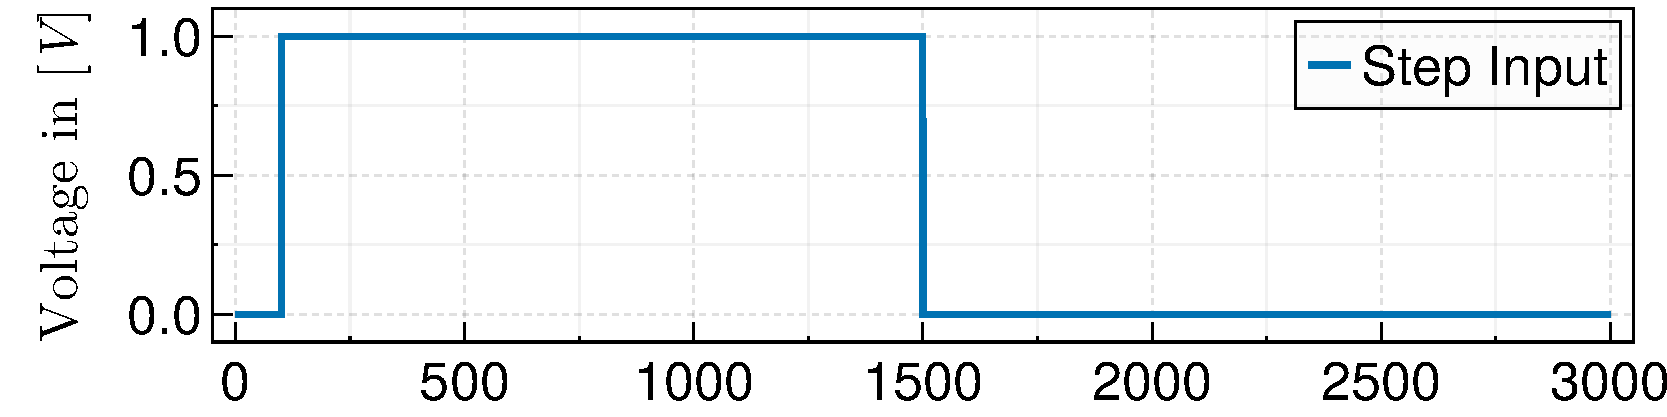
\includegraphics[width=0.95\columnwidth]{images/step_signal}}
	
	\subfloat[Capacitor]{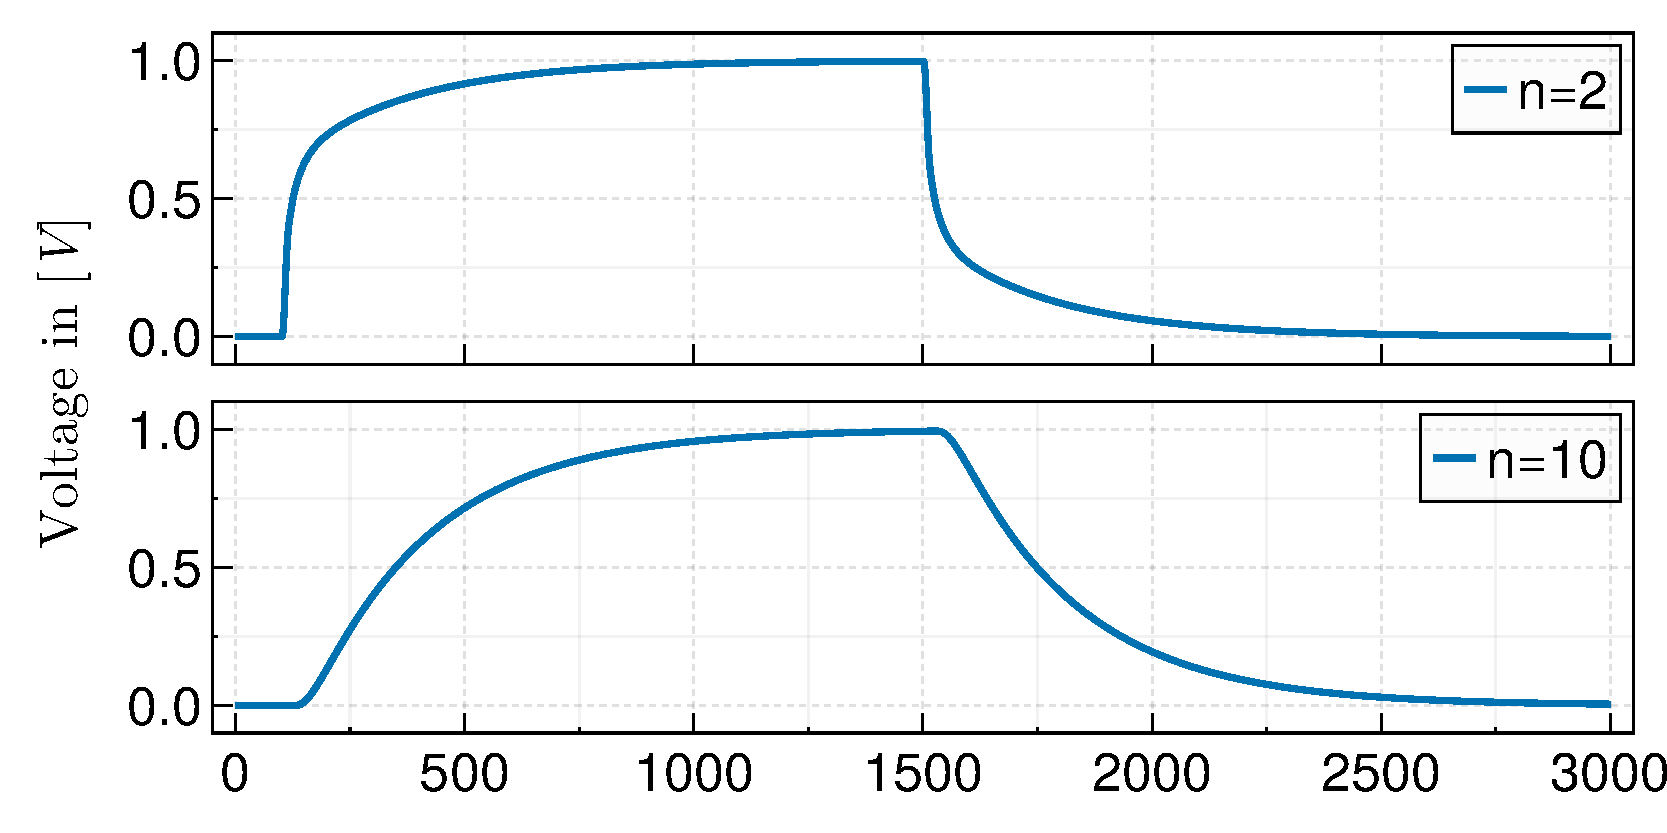
\includegraphics[width=0.95\columnwidth]{images/step_shunt_capacitor}}
	
	\subfloat[Resistor]{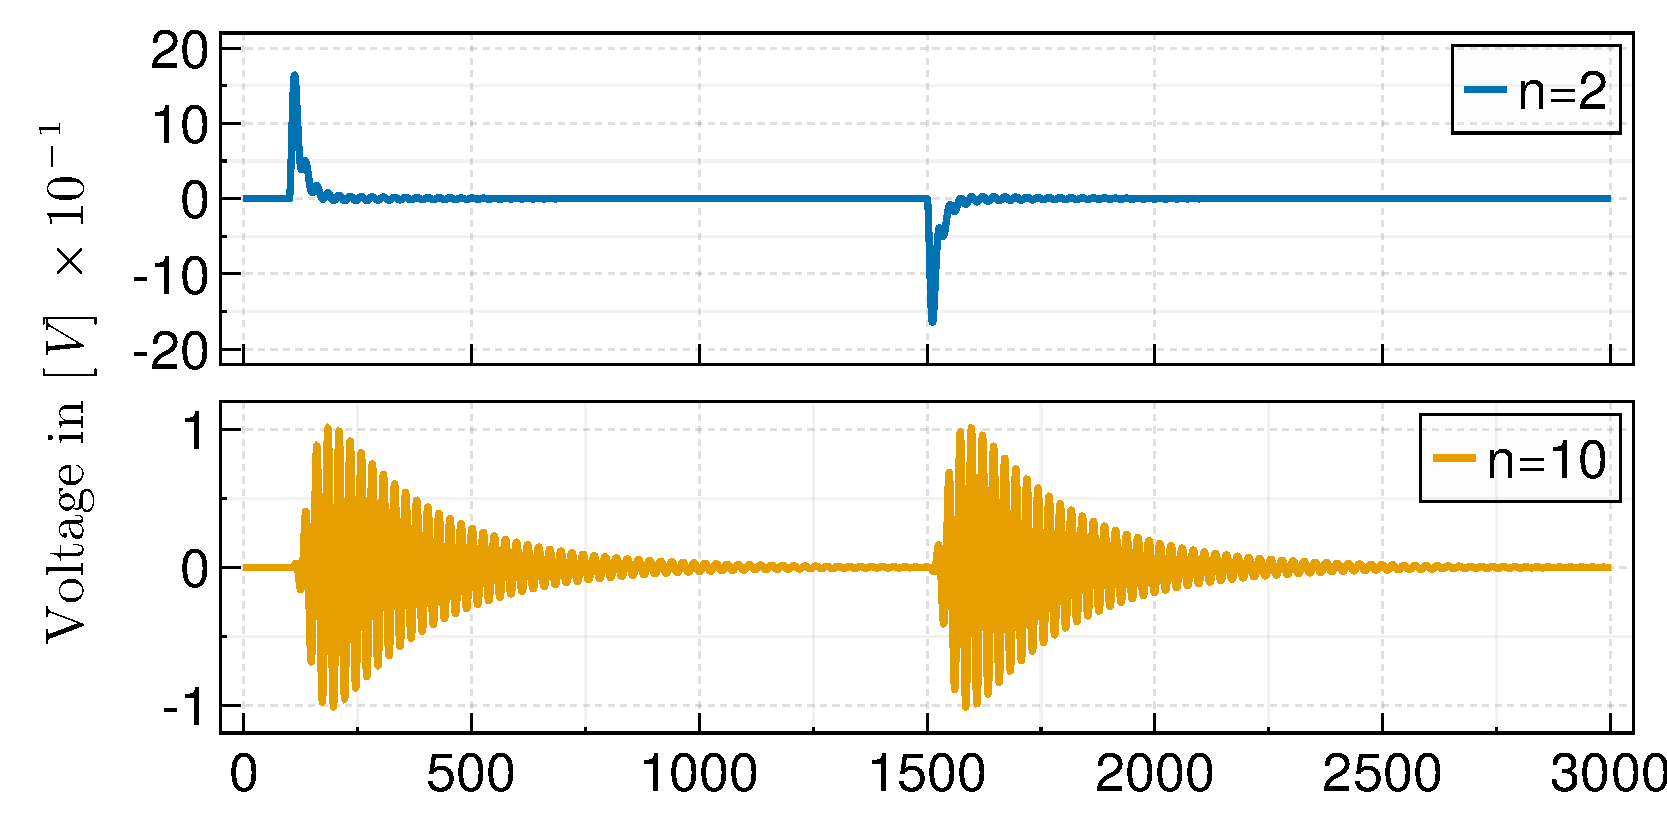
\includegraphics[width=0.95\columnwidth]{images/step_shunt_resistor}}
	
	\subfloat[Inductor]{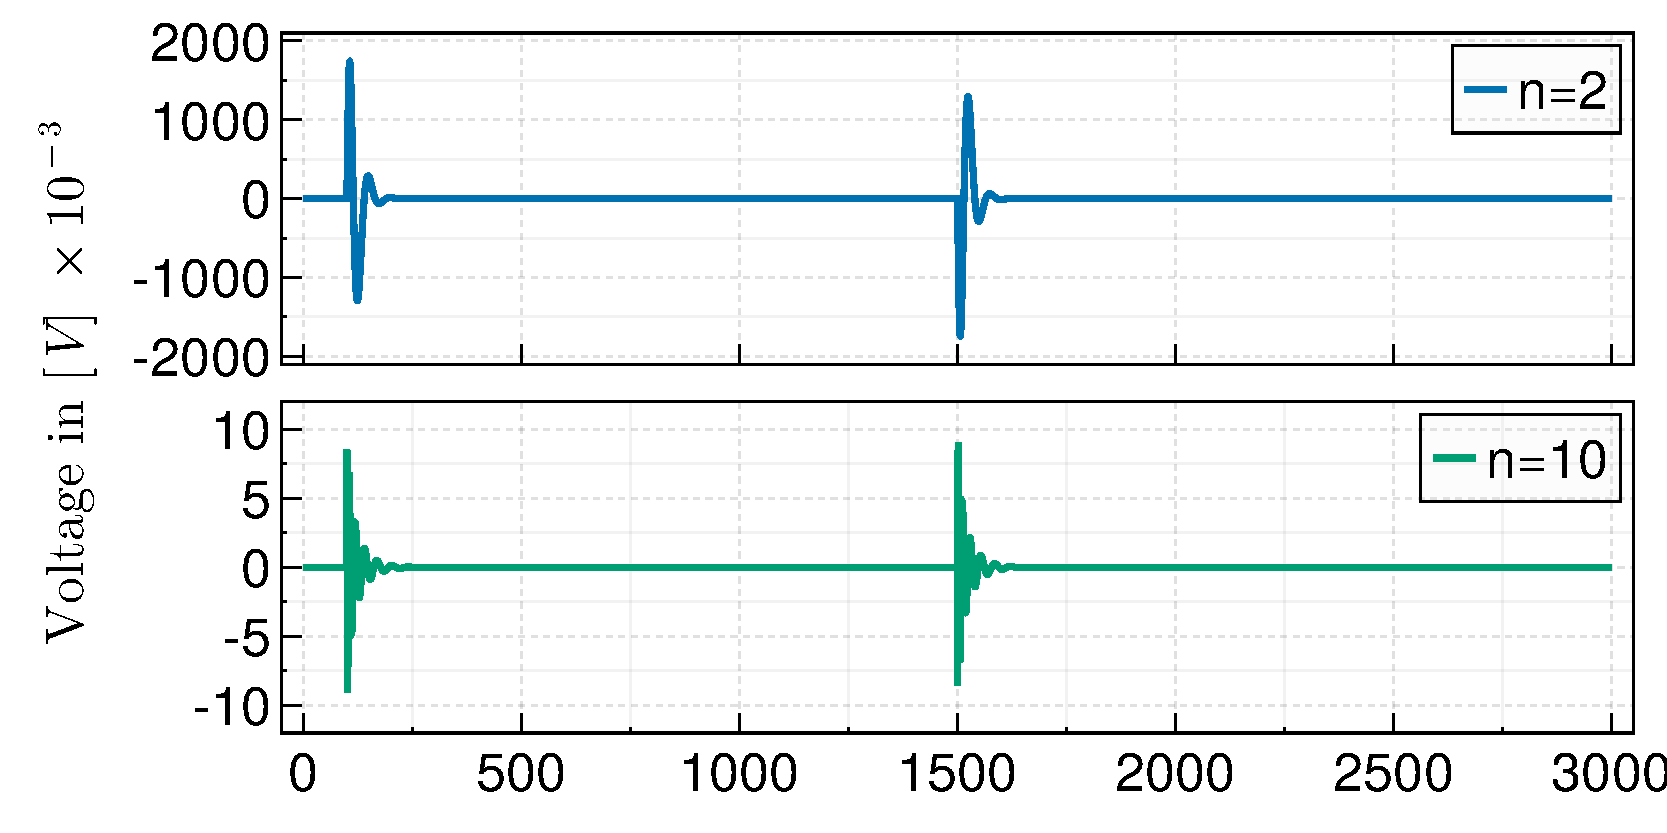
\includegraphics[width=0.95\columnwidth]{images/step_shunt_inductor}}
	
	\caption{Input signals and resulting states for Capacitor, Resistor and Inductor.}
	\label{fig:step_input_output_results}
\end{figure}	




\subsection{Symmetric Sweep Input Signal}
In case of ladder type (b) and (c), see Fig. \ref{fig:cascaded_rlc_circuits}, we need to differentiate the input voltage once and twice. We consider a two-sided chirp signal which starts and terminates at zero Volt and its first and second derivative, see Fig. \ref{fig:input_output_results} (a). We design an oscillation 
\begin{equation}
	f(t,p) = \sin\left(p~\pi~g(t,p)\right) \label{eq:input_base_oscillation}
\end{equation}
and with an embedded function
\begin{equation*}
	g(t,p) := \tanh\left(\frac{t}{p}\right)
\end{equation*}
We choose further $p=100$ and shift the time by $t \rightarrow t-700$ to yield the original voltage signal
\begin{equation*}
	u(t) = f(t-700,100) \textbf{.}
\end{equation*}
We differentiate symbolically the oscillation function, Eq. \eqref{eq:input_base_oscillation}, once to yield the first derivative
\begin{equation*}
	\partial_{t} f(t,p) = ~ \pi~\cos\left(p~\pi~g(t,p)\right)~ \left[1-g(t,p)^2\right]
\end{equation*}
and twice for the second derivative
\begin{align*}
	&\partial_{t}^2 f(t,p) =~ -\pi^2 ~ \sin\left(p~\pi~g(t,p)\right) ~ \left[1-g(t,p)^2\right]^2 \nonumber \\
	&\qquad - 2\frac{\pi}{p}~\cos\left(p~\pi~g(t,p)\right)~\left[g(t,p)-g(t,p)^3\right]
\end{align*}
Again, we set $p=100$ and the time shift as above for the first and second derivative to yield $\partial_{t} u(t)$ and $\partial_{t}^2 u(t)$.

%\begin{align*}
%	u(t) = f(t-700,100) \\
%	\dot{u}(t) = \partial_{t} f(t-700,100) \\
%	\ddot{u}(t) = \partial_{t}^2 f(t-700,100) 
%\end{align*}

\begin{figure*}[t!]
	\centering
	\subfloat[Input Signals]{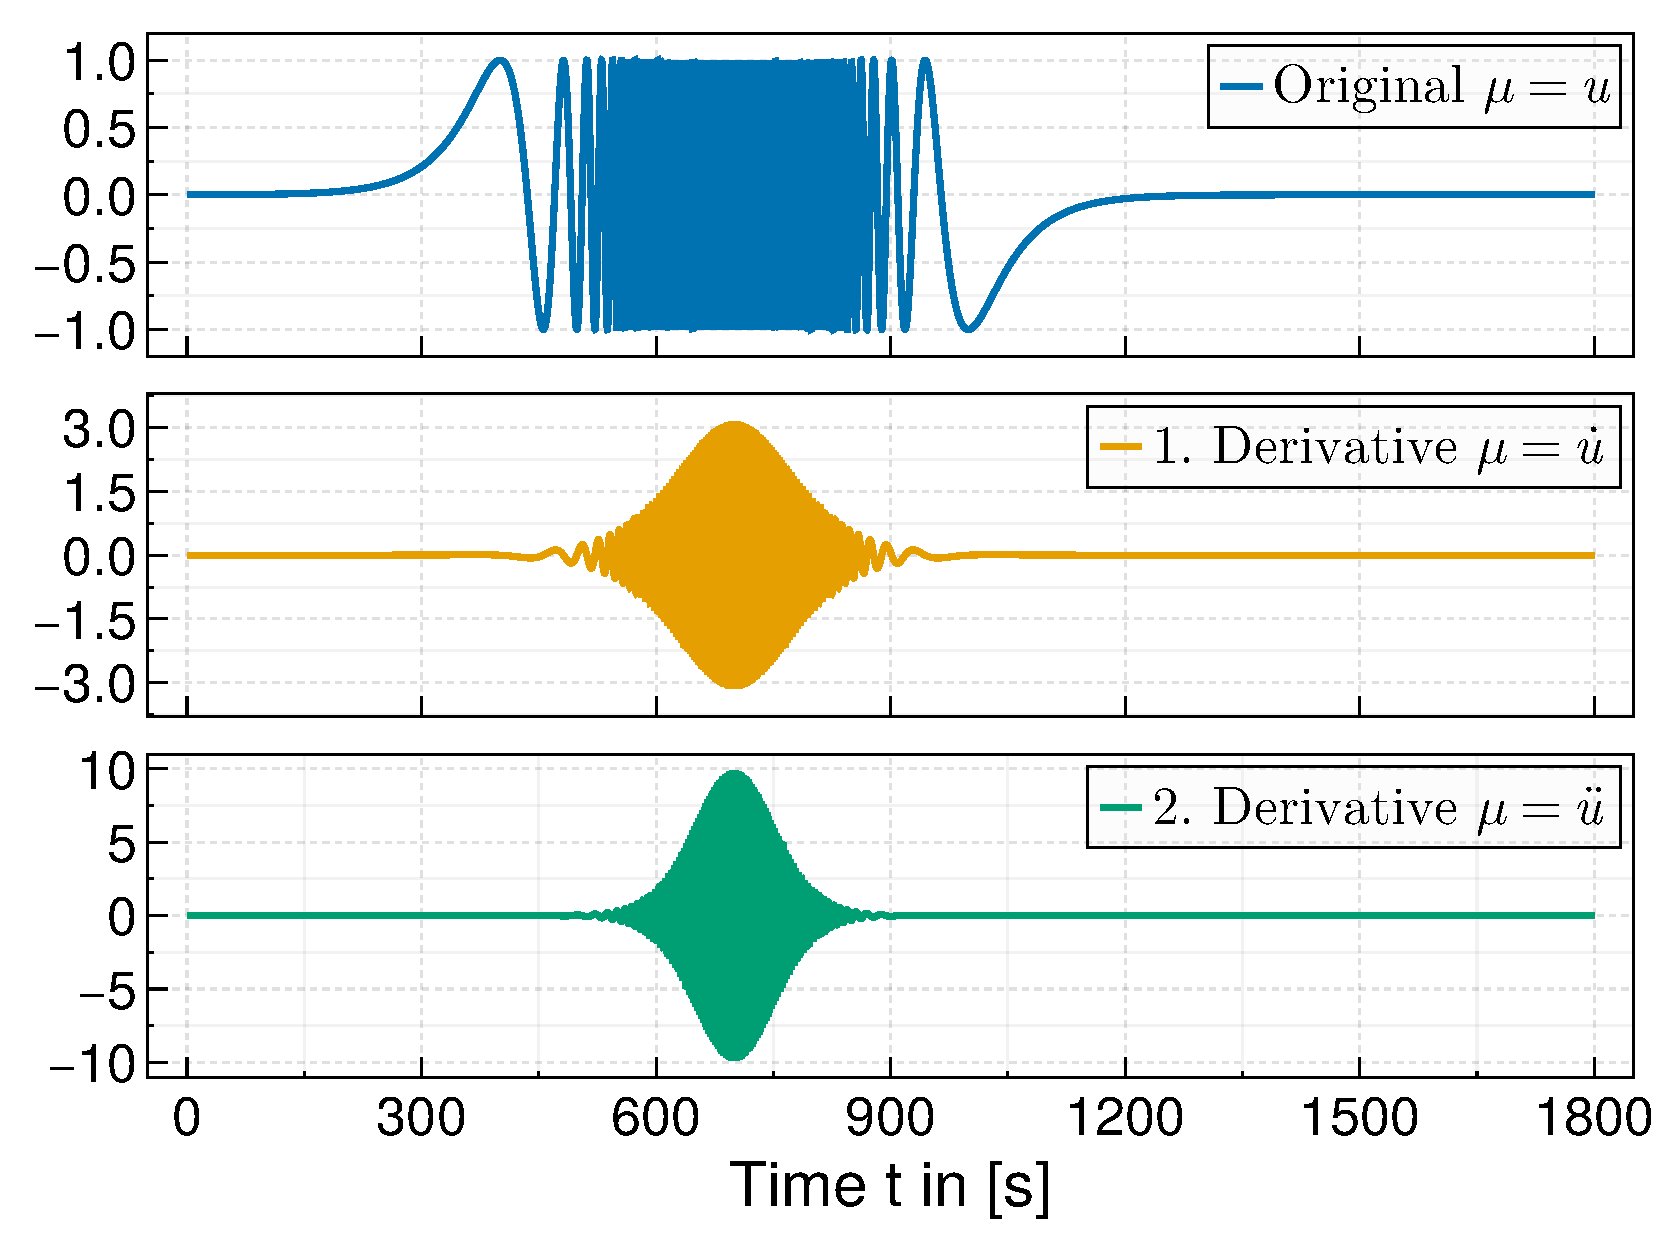
\includegraphics[width=0.47\columnwidth]{images/input_signal}}
	\hfill
	\subfloat[Capacitor]{
\includegraphics[width=0.47\columnwidth]{images/lines_shunt_capacitor}}
	
	\subfloat[Resistor]{
\includegraphics[width=0.47\columnwidth]{images/lines_shunt_resistor}}
	\hfill
	\subfloat[Inductor]{
\includegraphics[width=0.47\columnwidth]{images/lines_shunt_inductor}}
	
	\hfill
	
	\hfill
	

	\caption{Input signals and resulting states for Capacitor, Resistor and Inductor.}
	\label{fig:input_output_results}
\end{figure*}	


